\section{Discussion}
\begin{figure}[!t]
    \centering
    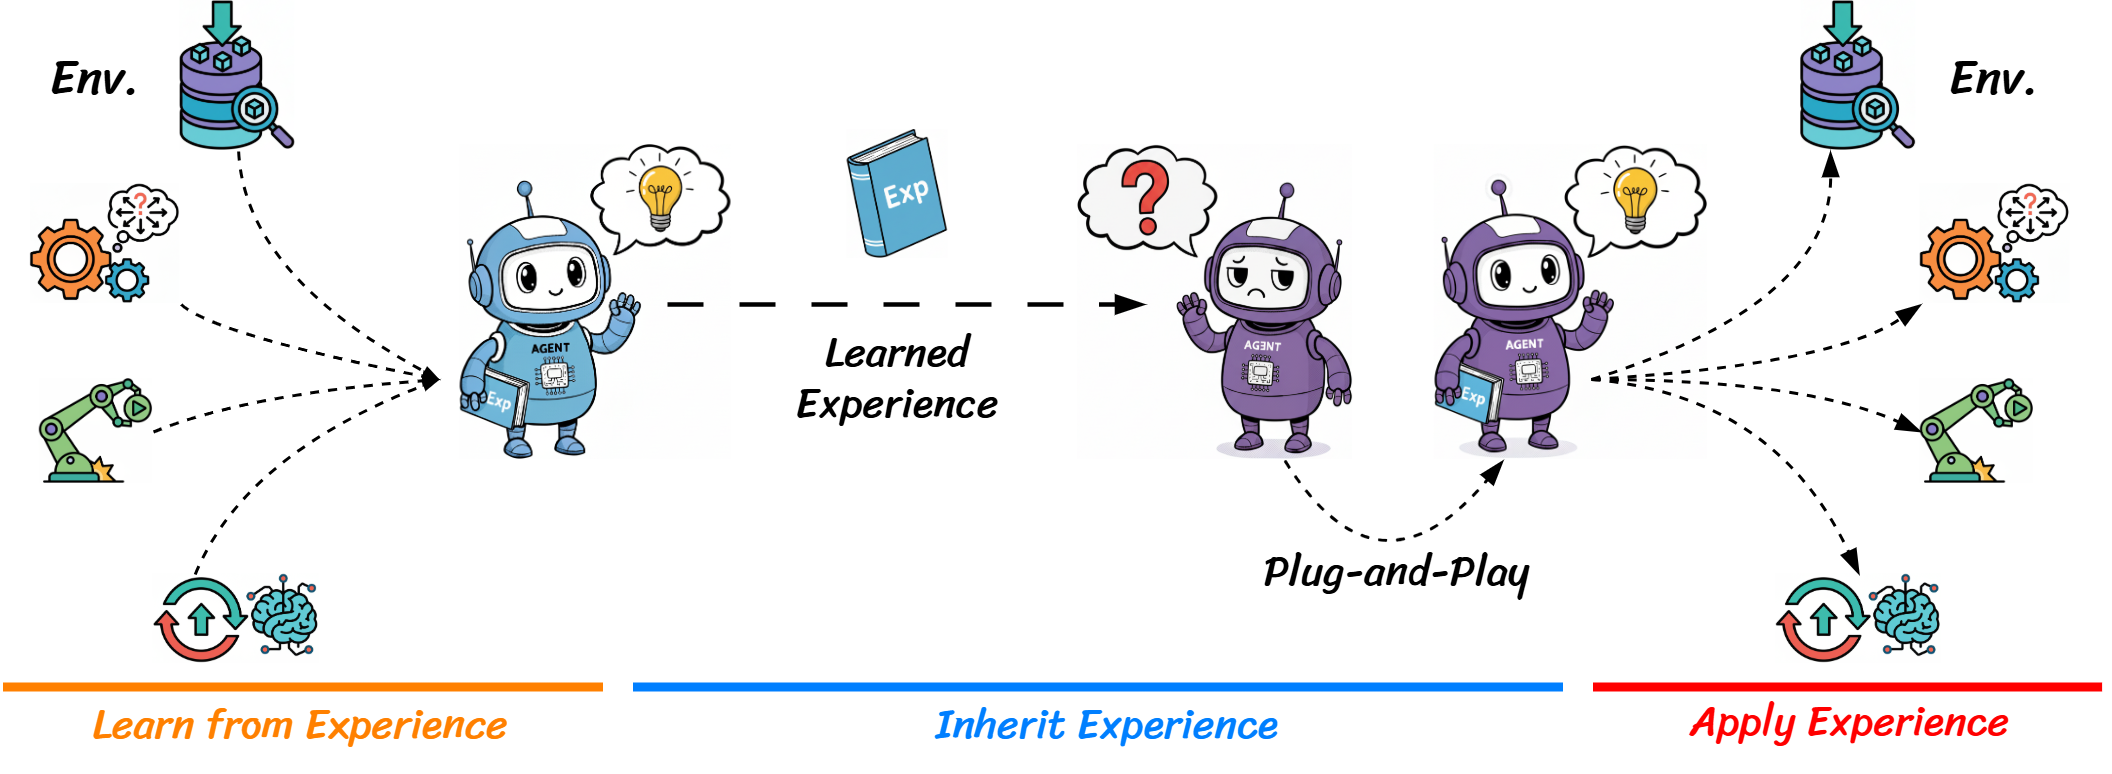
\includegraphics[width=\linewidth]{figs/inheritance.png}
    \caption{The process of inheriting the experience library across diverse agents. The experience library acts as a plug-and-play module that can boost agents' performance with a single training procedure.}
    \label{fig:inheritance}
\end{figure}

The aspiration to create intelligent agents that evolve through lived experience is a long-standing and central theme in artificial intelligence~\cite{turing2009,Russell2021AIMA}. This discussion aims to connect our research to this enduring quest, reflecting on the potential futures it might suggest and the historical context from which it emerges. We hope to offer a thoughtful perspective on the path ahead, framing our contributions not as conclusions, but as a humble step in an ongoing, collective journey.

\paragraph{Toward Continuous Learning.}
A central goal in AI is to enable agents to learn continuously from their interactions, much like living organisms do~\cite{sutton2023albertaplanairesearch,wang2024comprehensivesurveycontinuallearning}. This pursuit hints at a future where AI systems are not static artifacts, but dynamic partners capable of adapting in real time. For years, the research community has explored various avenues toward this goal, often seeking learning paradigms that are more "forward-looking" than traditional back-propagation~\cite{hinton2022forwardforwardalgorithmpreliminaryinvestigations}. The semantic capabilities of modern LLMs~\cite{openai2025gpt5,anthropic2025sonnet4.5,anthropic2025claude4,xai2025grok4}, however, offer a new lens for this quest. It becomes possible to explore learning not only as a numerical optimization task but as a process of reasoned reflection. Our explorations in this work suggest this is a worthwhile direction, raising the possibility for a new generation of AI systems whose learning processes are inherently more auditable and aligned with a lifelong learning model.

\paragraph{Heading to a Collective Wisdom.}
Beyond individual capability, another grand challenge is fostering a form of collective intelligence, mirroring how human progress is built upon shared knowledge~\cite{10.1145/3368986}. One can envision a future where a global network of specialized agents collaborate, forming a collective scientific mind to accelerate progress on humanity's greatest challenges. A key historical obstacle to this vision has been the absence of a robust medium to inherit wisdom across distinct AI agents~\cite{CAMPBELL200257,silver2017masteringchessshogiselfplay}. The concept of decoupling learned experience from an agent's internal parameters represents a hopeful path forward. Our explorations in this direction (Fig~\ref{fig:inheritance}) suggest that distilled experience can indeed serve as a viable medium for inheritance, adding a small contribution to the larger effort of building a foundation upon which a more synergistic AI ecosystem might one day be built.

\paragraph{Learning in a transparent way.}
Integral to the future of AI is the development of systems whose reasoning is transparent. This points toward a future where human-AI collaboration is built on a foundation of shared understanding, which is crucial for their integration into critical societal functions. The "black box" nature of many deep learning models has presented a persistent barrier to this goal~\cite{https://doi.org/10.1002/ail2.61,gohel2021explainableaicurrentstatus,hsieh2024comprehensiveguideexplainableai}. An experience-driven learning paradigm inherently addresses this challenge. When an agent's growth is chronicled as a series of explicit, human-readable experiences, its evolution becomes an open book. This transparency provides a direct mechanism for meaningful human-in-the-loop interaction~\cite{Wu_2022}, allowing experts to understand, guide, and even enrich an agent's learning journey. It represents a step toward a more white-box model of AI development, where the process of learning is as important as the final performance.

In conclusion, the ideas explored here are offered as a contribution to an ongoing conversation. It is our sincere hope that this work serves as one humble effort for the field, contributing to a future where AI evolves as a more dynamic, collaborative, and transparent partner in the human endeavor.